%-----<<< PROBLEM DEFINITION >>>-----
\chapter{Problem Definition}
\label{ch:problem}

This chapter formulates more precisely the problem we are solving, and provides information about the design of our FWMAV, as well as the experimental setup.
The intended mission of the vehicle is to continuously follow an arbitrary trajectory. The trajectory is represented as a set of waypoints connected in straight lines. The trajectory is pre-defined and static during the mission. The vehicle will determine what is the best way towards the next waypoint and what control action needs to be taken to get there. The mission ends after reaching the last waypoint. In case obstacles are present, the vehicle is required to avoid them autonomously and resume the desired trajectory. The biggest challenge is the allocation of the control inputs, i.e. finding out what control action is needed. The vehicle is also required to automatically recover from faults that could occur during the mission, such as wing damage and control system malfunction. 

\section{Vehicle Configuration}
\label{sec-vehicle-configuration}

A conceptual vehicle closely related to those described by Wood~\cite{Wood2008},~\cite{robobees} and Doman~\cite{afrl1},~\cite{afrl2}, is presented in \cite{gallagher}.
Our vehicle is an upgraded version of a FWMAV described in~\cite{Perseghetti}~\cite{Boddhu}~\cite{Botha} and has two wings providing all propulsion and control forces.

It approximates a passively upright-stable version of the vehicle from \cite{gallagher} operating near its hover wing flapping frequency. The wings are mounted in the $Y_b$--$Z_b$ body plane (see Figure~\ref{fig:fwmav}). These wings are actively actuated within the range of $\pm\phi$ radians. As the spars rotate, dynamic air pressure lifts the triangular wing platforms (membranes) up to an angle of $\alpha$ radians under a base vector embedded in the $Y_b$--$Z_b$ plane. Individual wing flaps produce independent lift and drag forces at each of the two wing roots (points of attachment of the wings to the body). These can be resolved into body frame forces and torques and cause changes in the whole vehicle’s position and pose in three-dimensional space.

\begin{figure}
\centering
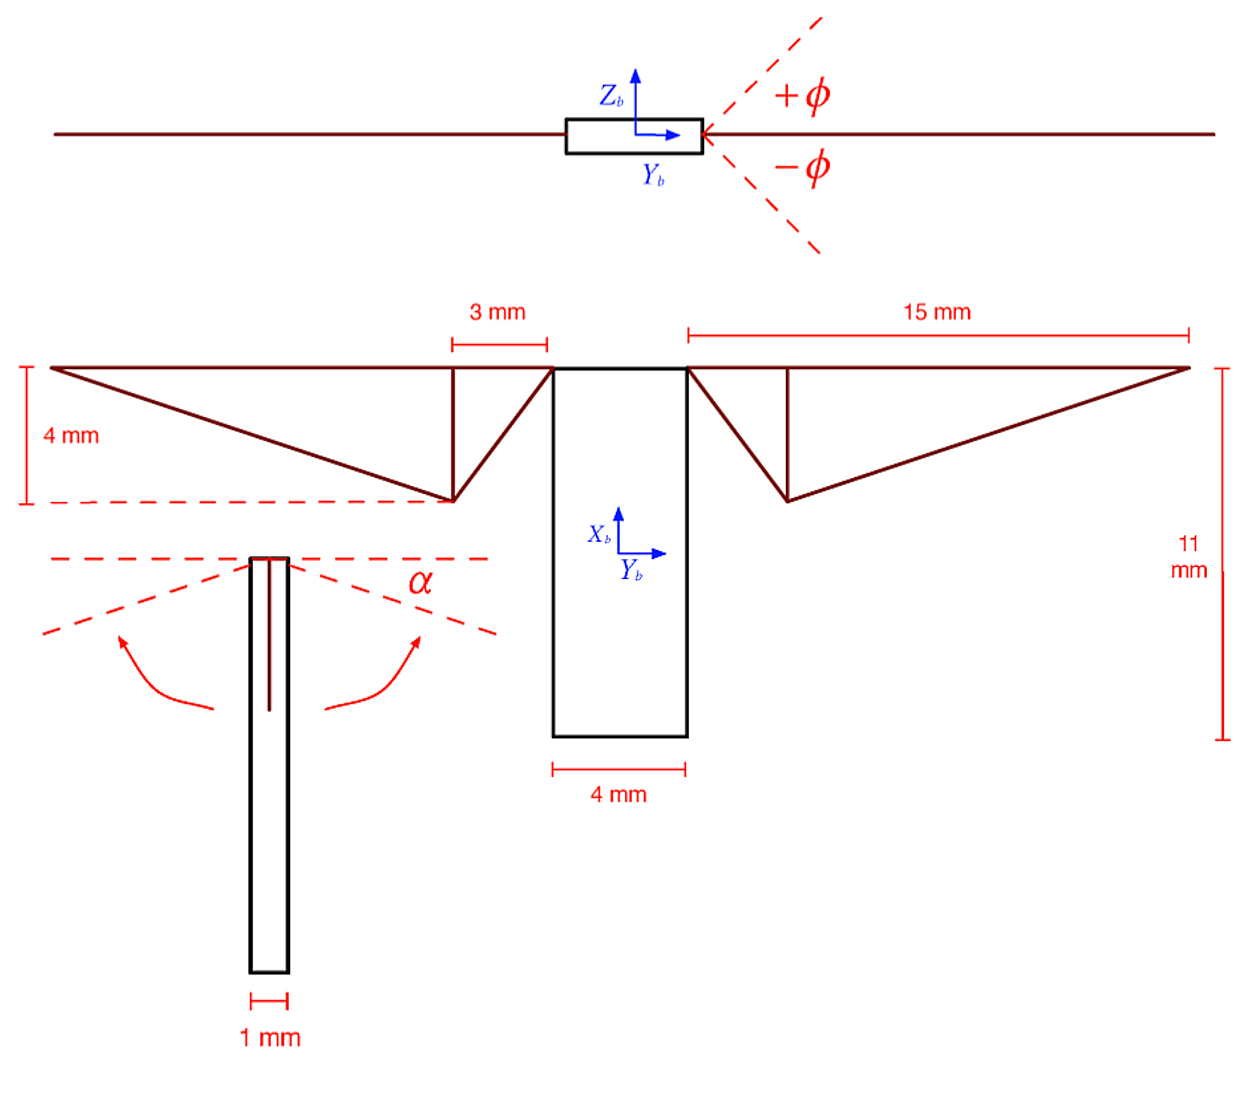
\includegraphics[width=0.64\textwidth]{Files/Figures/fwmav.png}
\caption[Orthographic view of flapping wing vehicle]{Orthographic view of a FWMAV \cite{gallagher}. Both wing spars are restricted to rotational motion about their joints with the body and in the $Y_b$--$Z_b$ plane. The range of those rotations is [$-1\ldots1$] radians, $\alpha$ is between $\pi/6$ and $\pi/2$ radians. Note that the dimensions are for orientation purposes only, and differ on the actual vehicle which is larger.}
\label{fig:fwmav}
\end{figure}

\section{Cycle Averaged / Split Cycle Control}
\label{sec-splitCycleControl}

The cycle averaged control is based on estimates of what forces a wing would produce, on average, over a single wing beat. For example, a cycle-averaged altitude controller might compute the error between current and desired altitude, use an error feedback control law to compute the desired force to apply to the body, and finally use a model of the vehicle's wings to compute the parameters of a single wing beat that, when adopted by both wings, produces the desired force (on average) during the whole wing beat. Cycle-averaged control wraps a feedback control law around the whole wing beat as an atomic constructs rather than around finer-scaled micro-motions of wings. The desired wing motions are "communicated" to the wings once per wing beat as a small number of shape parameters that define how the wing will move during that wing beat.

\textit{Split-cycle control} is a special case of cycle-averaged control in which wing beats are composed of two half-cosine waves, one each to govern the wing's upstroke (front to back) and downstroke (back to front). The shape parameters communicated to each wing are a flapping frequency ($\omega$~[rad/s]) and an upstroke/downstroke transition parameter ($\delta$~[rad/s]). Advancing the upstroke (and consequently impeding the downstroke) produces a forward force while keeping the wing beat frequency constant. Formally, $\phi_U = \cos( (\omega - \delta)t)$  and $\phi_D = \cos( (\omega + \sigma )t)$ where $\sigma$ is dependent on $\delta$. From \cite{afrl2} we know that $\delta \in [-\infty \ldots\omega /2]$ although certain value ranges are particularly important. If $\delta = 0$ the upstroke is symmetrical to the downstroke and a regular wingbeat occurs. However, if $\delta>0$ the upstroke is impeded and the downstroke is advanced, as shown in Figure~\ref{fig_deltaPlus}. As a result, a force is generated in the direction of the downstroke. Conversely, if $\delta<0$ then the downstroke is impeded and the upstroke is advanced, as shown in Figure~\ref{fig_deltaMinus}, resulting in a force in the direction of the upstroke. These lateral forces act on the vehicle's body via a moment arm producing an angular momentum. Put simply, by applying the split cycle the vehicle can turn. See \cite{afrl2} for a derivation and a proof of split-cycle operation.

A conventional application of a split-cycle control to our vehicle might entail an "outer loop" of multiple body axis controllers (e.g., one that computes altitude error and determines a flapping frequency for the wings, one that computes a roll axis angle error and computes antagonistic shifts to produce a roll moment, etc.), and an allocator that harmonizes all of the flapping frequency and shift commands made by the various axis controllers for presentation to an "inner loop" controller that would ensure the wings follow the correct cycle averaged trajectories. Control would then consist of an outer loop that, based on vehicle state, provides $\omega$s and $\delta$s that should produce forces required to effectively correct position and pose errors and an inner loop that, receiving those $\delta$s and $\omega$s, would ensure the wings moved as required.

\begin{figure}
\centering
\minipage{0.49\textwidth}
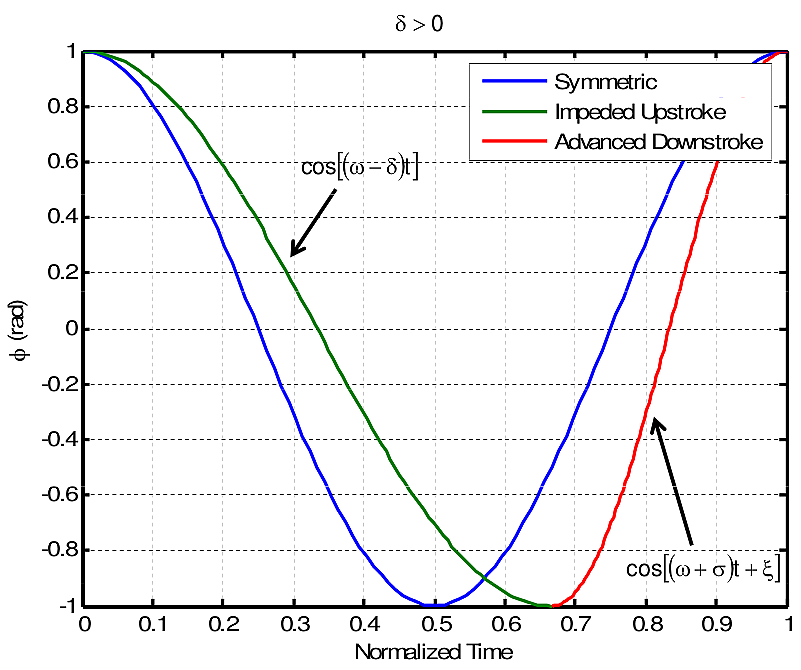
\includegraphics[width=\textwidth]{Files/Figures/deltaPlus.png}
\caption[Split-cycle results for $\delta > 0$]{Split-cycle results for $\delta > 0$}
\label{fig_deltaPlus}
\endminipage\hfill
\minipage{0.49\textwidth}
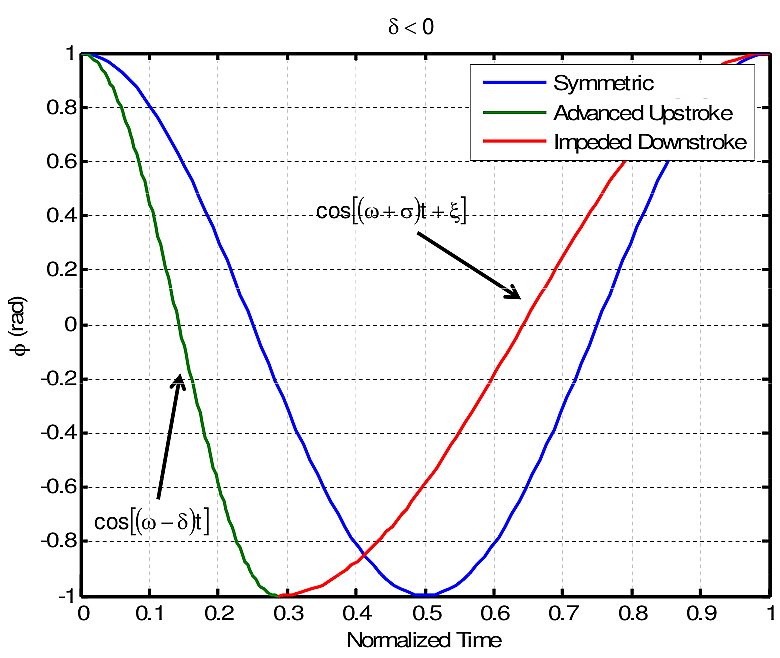
\includegraphics[width=\textwidth]{Files/Figures/deltaMinus.png}
\caption[Split-cycle results for $\delta < 0$]{Split-cycle results for $\delta < 0$}
\label{fig_deltaMinus}
\endminipage\hfill
\end{figure}


\section{Experimental Setup and Environment}
\label{sec-environment}

All experiments are to be conducted in a large ($5' \times 5'$) water tank. The vehicle is restricted move on a two-dimensional plane and rotate around its $X_b$ axis, which simulates operation around hover. The vehicle consists of a pair of wings (shown in Figure~\ref{fig_wings} and is equipped with a pair of Lithium Polymer batteries, a power distribution board and a main computer, as shown in Figure~\ref{fig_robot}. All hardware is mounted on a carbon-fiber platform, attached to a floating Styrofoam puck, which keeps the robot on the surface. The water surface acts as a mechanical low-pass filter, slowing down the vehicle movement and dampening disturbances, which allows us to test our control system without the need for expensive high-speed cameras. A camera is placed above the water tank, so its field-of-view encompasses the entire water tank. The camera locates and records the vehicle position. A sample capture view from the camera is shown Figure~\ref{fig_robotInActionTop}.

\begin{figure}
\centering
\minipage{0.49\textwidth}
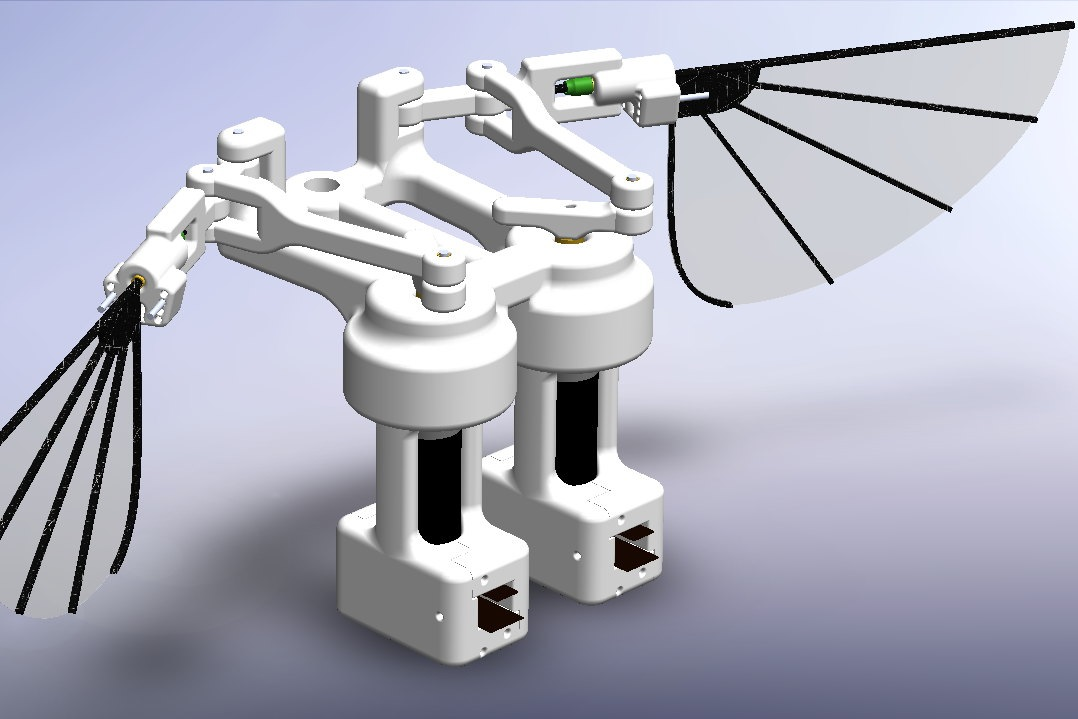
\includegraphics[width=\textwidth]{Files/Figures/wings.jpg}
\caption[3D model of wings]{3D model of wings with linkages and motors. Video showing moving wings is available from \cite{cpsgroup} \newline}
\label{fig_wings}
\endminipage\hfill
\minipage{0.49\textwidth}
\center
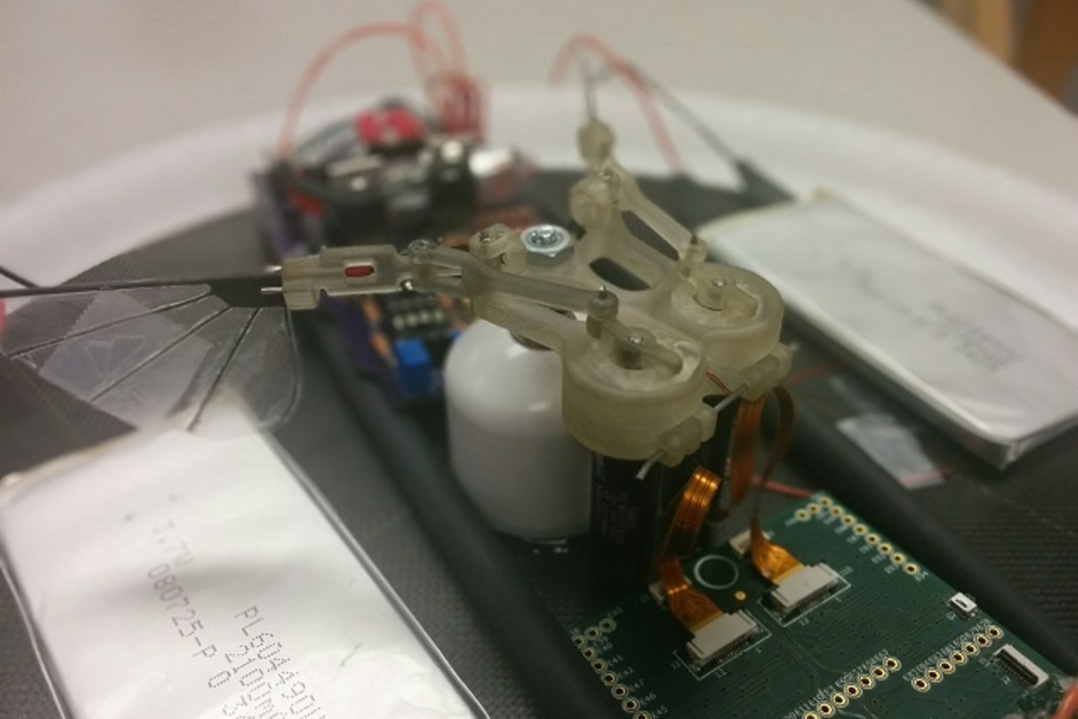
\includegraphics[width=\textwidth]{Files/Figures/robot.jpg}
\caption[Assembled vehicle]{Assembled vehicle---note wings in the middle, LiPo batteries on sides, the power distribution board in the back and the control board in front.}
\label{fig_robot}
\endminipage\hfill
\end{figure}

\begin{figure}
\centering
\minipage{0.49\textwidth}
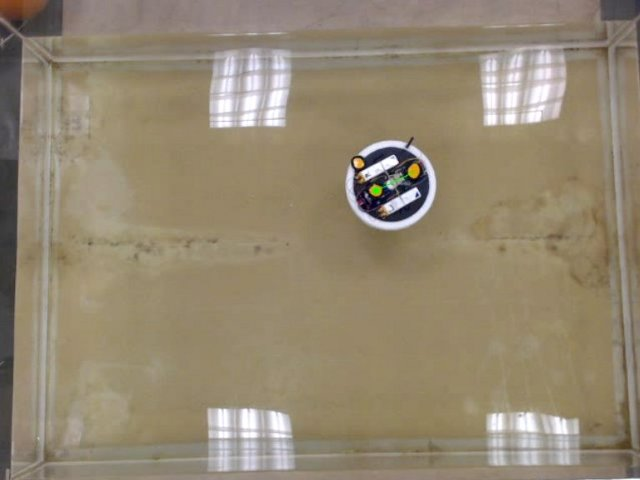
\includegraphics[width=\textwidth]{Files/Figures/watertank.jpg}
\caption[Vehicle during an experiment in the water tank (top-view)]{Vehicle during an experiment in the water tank (top-view). Note the color markers used for machine vision pose estimation. The four white squares are reflections of the ceiling lights and are not related to the experiment.}
\label{fig_robotInActionTop}
\endminipage\hfill
\minipage{0.49\textwidth}
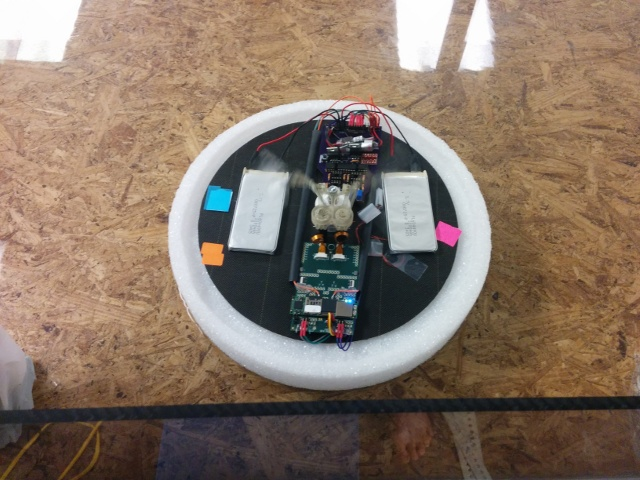
\includegraphics[width=\textwidth]{Files/Figures/robot2.jpg}
\caption[Vehicle during an experiment in the water tank (close-up view)]{Vehicle during an experiment in the water tank (close-up view). Note the color markers used for machine vision pose estimation.\newline \newline}
\label{fig_robotInActionClose}
\endminipage\hfill
\end{figure}

During the development of the image processing pipeline that reliably tracks the vehicle in the whole area of the water tank we examined a number of different approaches:
\begin{enumerate}
\item \textbf{Color Markers} - using color markers of specific color and dimensions is a very common method, but suffers from changing light conditions. Typically the image is converted into HUV (Hue-Saturation-Value) color space because it is more robust than RGB color space, and then filtered so only the markers are left in the image. The position and orientation is then calculated using a simple geometry. Figure~\ref{fig_robotInActionClose} shows the robot with color markers.
\item \textbf{Lukas Kanade Tracker (LKT)}\cite{Lucas1981} -- LKT uses optical flow (mentioned in Section~\ref{subsec:vision_based_sensors}) to track an object within the image. LKT needs a template of the object to start with (for example an image of the robot), but can track changing object (i.e. when the lighting changes), which would be suitable for our application. Unfortunately LKT by itself cannot determine the orientation of the object, which means we would know only position of the robot. To obtain orientation, additional methods need to be used.
\item \textbf{SURF feature matching} -- SURF detector \cite{Bay2008} finds suitable features in the image, that can subsequently be matched by FLANN based matcher \cite{Muja09fastapproximate}. Once the match between the original object and the template is established, homography can be calculated using RANSAC algorithm \cite{Fischler}, which is then used to calculate the pose of the robot - an example of this process is shown in Figure~\ref{fig:vision_matching}. The drawback is higher computational complexity because of the matrix transformations involved.
\end{enumerate}


\begin{figure}
\centering
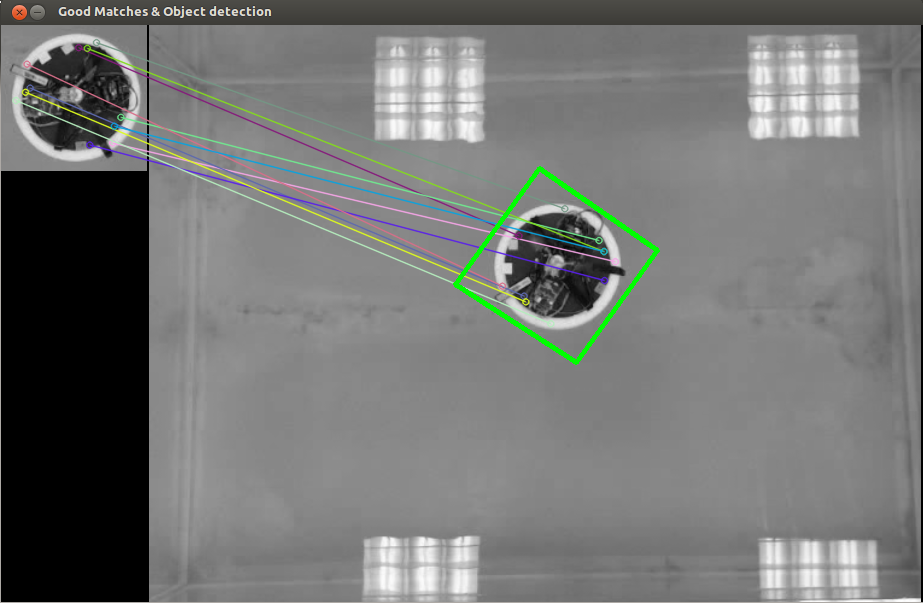
\includegraphics[width=0.8\textwidth]{Files/Figures/vision_matching.png}
\caption[Feature matching example]{An example of feature matching between a template picture (top left) and recorder camera image. The features found in both images are circled in color and connected by colored lines. The green square represents the calculated orientation and position of the robot (in this case roughly 60~deg counter clockwise)}
\label{fig:vision_matching}
\end{figure}


We combined the LKT with SURF detector and subsequent feature matching to provide a tracker capable of following the robot across the whole water tank (even when the vehicle was partially occluded), but because the pose was estimated incrementally (i.e. we were looking at the pose difference from the last estimated pose) the algorithm suffered from integration errors and as a result drifted in orientation estimate. Running algorithm is shown in Figures~\ref{fig:surf1} and~\ref{fig:surf2}. These issues could have been indeed resolved, but since the computational complexity of the algorithm was already fairly high (around 100~ms to process one camera frame on a regular laptop), it wouldn't be viable for real-time tracking at 30~Hz and we opted out for a simpler approach using color markers. 


\begin{figure}
\centering
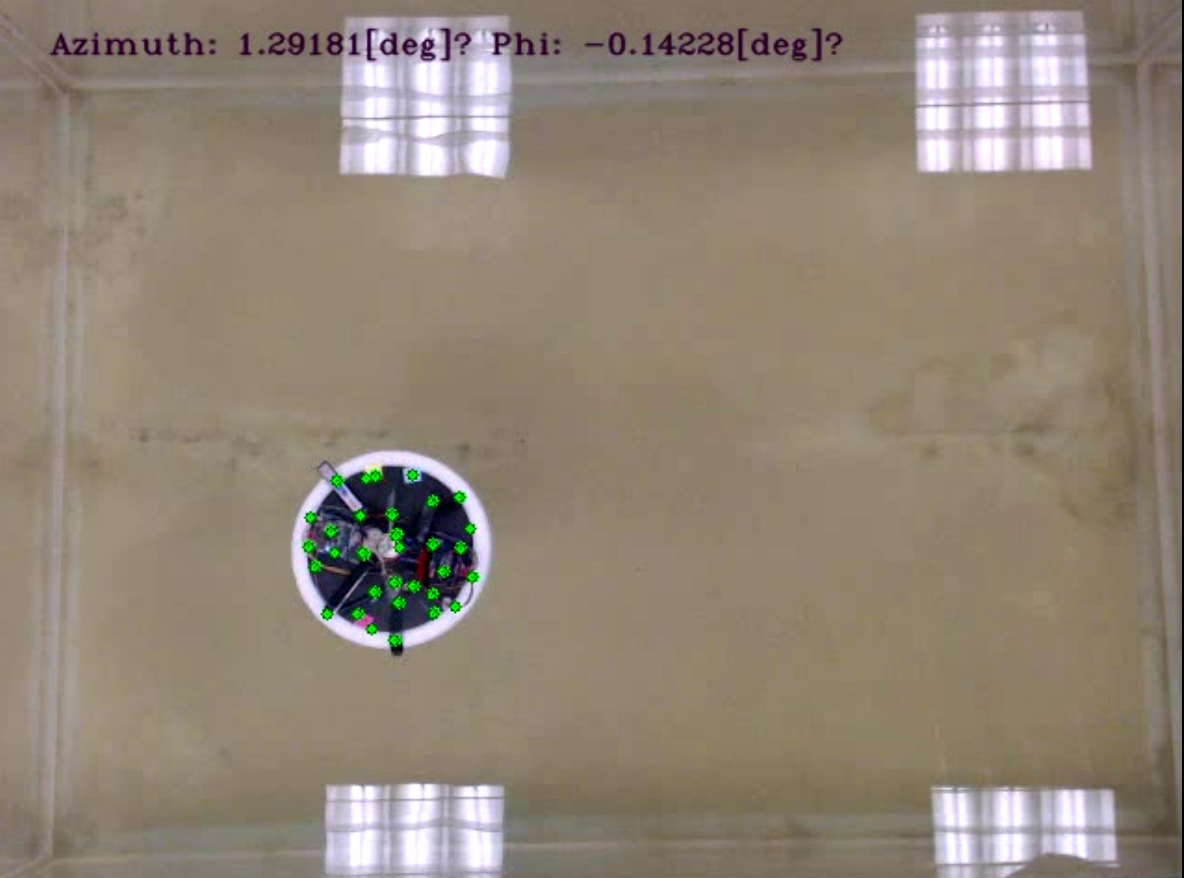
\includegraphics[width=0.8\textwidth]{Files/Figures/surf1.png}
\caption[Robot tracking - initialization]{An example run of the tracking algorithm based on LKT and SURF: Shortly after the initialization the azimuth estimate is precise (0~deg means the robot is facing directly towards the right)}
\label{fig:surf1}
\end{figure}

\begin{figure}
\centering
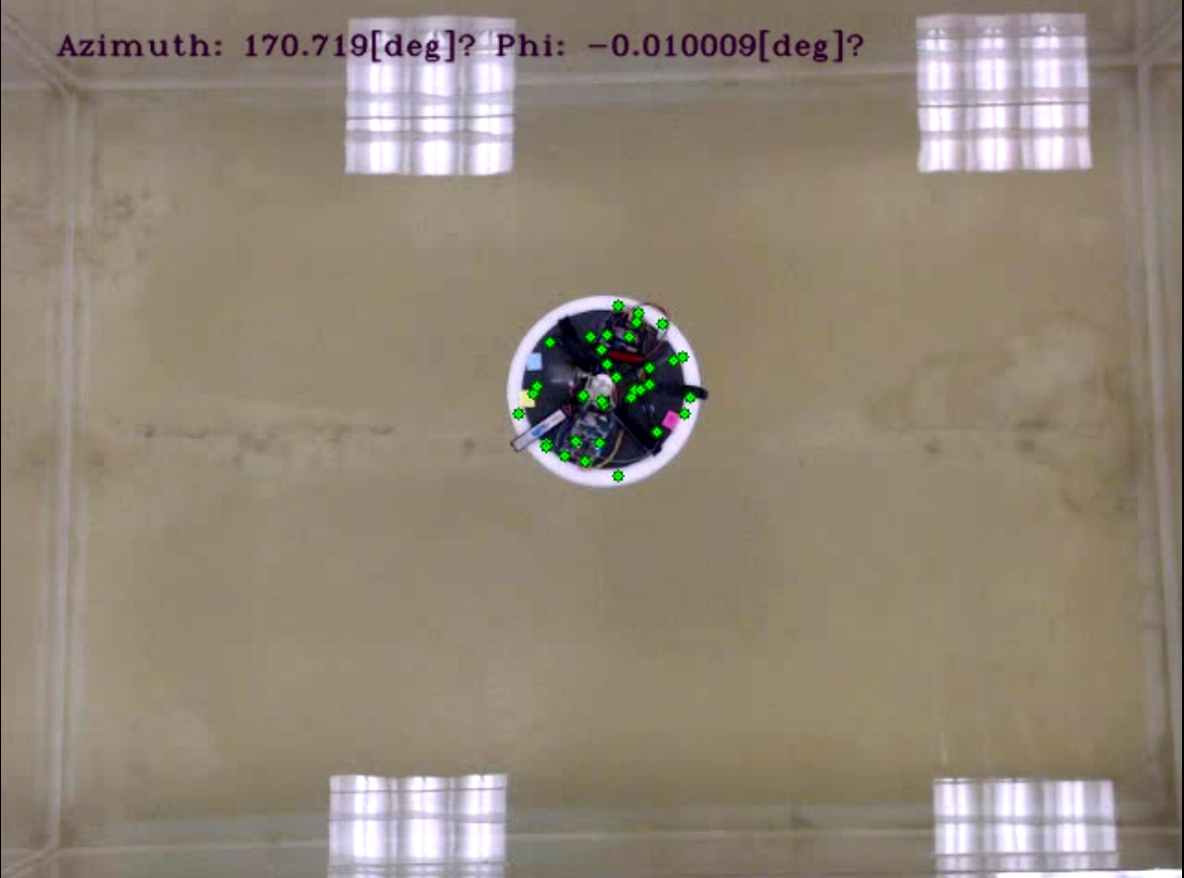
\includegraphics[width=0.8\textwidth]{Files/Figures/surf2.png}
\caption[Robot tracking - orientation drift]{An example run of the tracking algorithm based on LKT and SURF: As the integration error accumulates, the estimated azimuth quickly drifts. In this case the estimate is around 170~deg, while the true orientation is around 80~deg)}
\label{fig:surf2}
\end{figure}


After a careful calibration the markers were recognizable in most of the water tank, but in some places the light reflection leads to intermittent loss of tracking. Nonetheless the color markers worked reliable despite for our experiments despite this disadvantage. The processed video is recorded for reference, and the estimated pose is sent to the onboard MAS via a WiFi link.



\section{3D Printing \& Vehicle Assembly}
\label{sec-print}
The original parts for the vehicle were printed using a high-end industrial 3D printer. During the assembly and necessary repairs of the vehicle, it was needed to print additional spare parts. The 3D printing technology advanced very rapidly since the first prototype of the vehicle was built, and we were able to use successfully a consumer grade 3D printer (\textit{Mojo 3D}) to print all necessary linkages. Detailed 3D CAD models of the whole assembly are available, so the whole vehicle can be easily reproduced. %See Appendix~\ref{a:mechanical-design} for details.

In batch we can print enough parts for three pairs of wings. The price for one batch is around \$6. Figure~\ref{fig-3d-raw} shows the printed parts right after they were printed. The printing took around two hours. The printed parts have to be cleaned in a solution (to remove the support material), and in hand (to remove print imperfections). The cleaned parts are shown in Figure~\ref{fig-3d-cleaned}.

\begin{figure}
\centering
\minipage{0.49\textwidth}
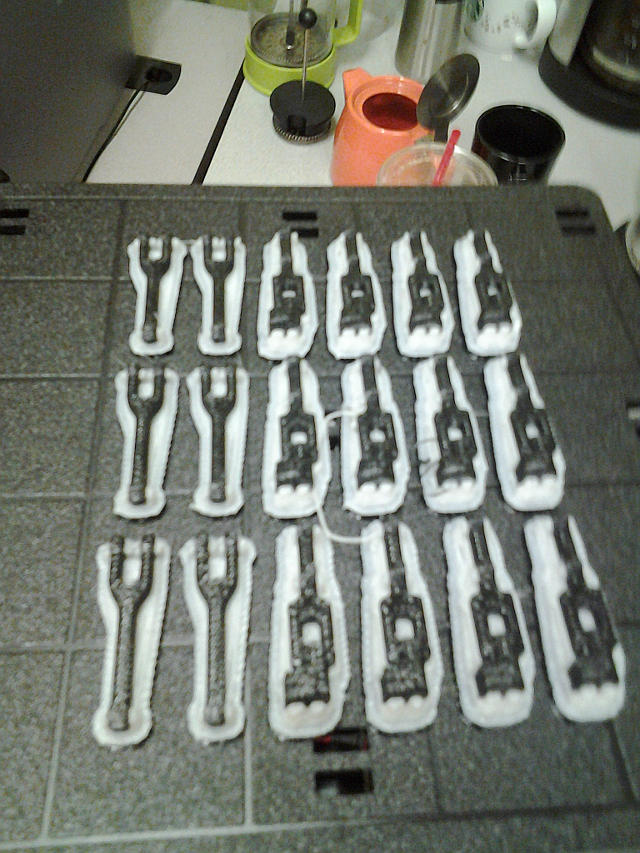
\includegraphics[width=0.9\textwidth]{Files/Figures/3d_printed_parts_from_printer_small.jpg}
\caption[3D printed parts]{3D printed parts. Notice the couplers on the left, and the left and right rockers on the right. Left and right rockers are identical.}
\label{fig-3d-raw}
\endminipage\hfill
\minipage{0.49\textwidth}
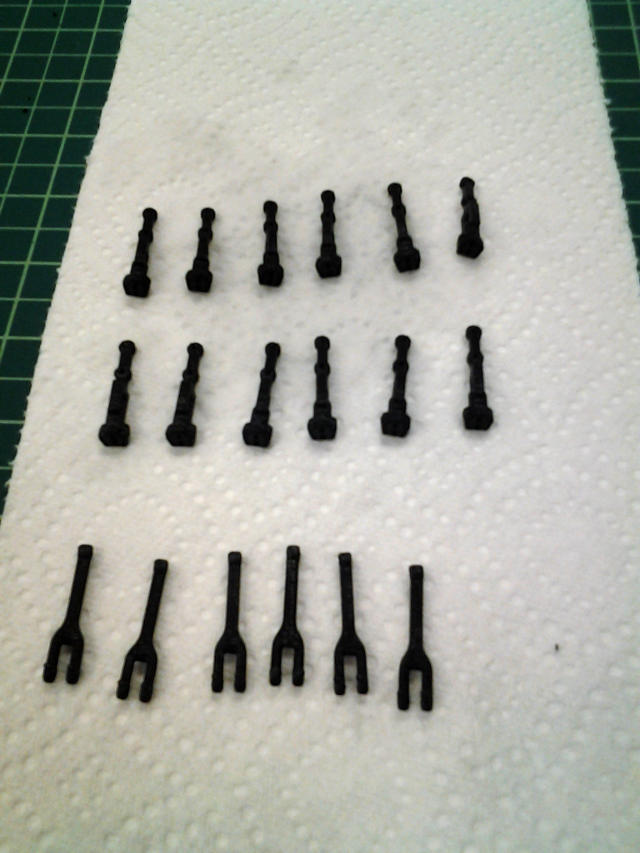
\includegraphics[width=0.9\textwidth]{Files/Figures/3d_printed_cleaned_parts_small.jpg}
\caption[3D printed parts after cleaning]{3D printed parts after cleaning.\newline \newline}
\label{fig-3d-cleaned}
\endminipage\hfill
\end{figure}

After the parts are cleaned, the wing linkage can be carefully assembled. It is a very tedious process, taking up a few hours. The individual parts have to be sanded off for a precise fit; sometimes the holes have to be cleaned with a hand drill and brass bushings have to be inserted to reduce friction between parts. Fortunately, the assembly and repair process is well documented, including a video with a detailed description of the process. 

We have shown that new parts can be printed very easily, and a multitude of wing assemblies can be put together relatively quickly, which is important because the ABS plastic isn't very rigid, quickly wears off and bends under stress, hence repair-ability is a crucial aspect of the design. The complete vehicle assembly, however, requires special motors, encoders and custom printed circuit boards and neither of those can be obtained quickly or cheap. More details about the vehicle, including part numbers, mechanical drawings and software architecture can be found in Appendix~\ref{a:mechanical-design}.


\section{Simulation}
\label{sec-sim}
A simulator of the vehicle is used for extrinsic evolution during initial learning (see Section~\ref{subsec-FirstStageAdaptation} for details). The simulator contains a simplified model of the vehicle with 3DOF -- a two-dimensional movement on the water surface plus a rotation around vehicle's z-axis. The simplified model assumes no external disturbances, such as wind. It assumes a perfect control over wing position (i.e. no slip in the linkages). It assumes a perfectly balanced vehicle, moving on a frictionless plane. The simulator, however, can be extended to include full 6DOF movement of a flying vehicle, and additional disturbances can be modelled too.

The simulator calculates cycle averaged lift and drag forces, meaning the produced lift and drag forces are averaged over one full wingbeat. The produced forces are then propagated to the body model, creating moments and change in orientation and position of the vehicle. Cycle averaged forces are a good approximation, because the low level controller cannot change the $\delta$ and $\omega$ parameters more often than at the beginning of the wing beat. As mentioned previously, the simulator is not intended to perfectly model the vehicle, but to provide a reasonably accurate initial values for the learning algorithms and their verification. 

The core of the simulator is a Java library containing vehicle dynamics model, and performing all necessary lift and drag calculations. The library was developed by the research group participating in this project. The agents are implemented using the MASON toolkit~\cite{mason}, which is also used as a visualization front end. The MASON toolkit is used to verify the MAS architecture---e.g. to make sure that the correct rules from the rulebase are firing in right order, and to check the correctness of the scheduler by moving the vehicle along predefined test trajectories. A screenshot of the running simulator is shown in Figure~\ref{fig:simulator}. Other robotics simulators, such as \textit{Gazebo}, could be used for modelling and simulation, but developing it was beyond the scope of this project.

The next chapter describes how we approached the problem and the MAS we designed, together with the fault recovery mechanism.

\begin{figure}
\centering
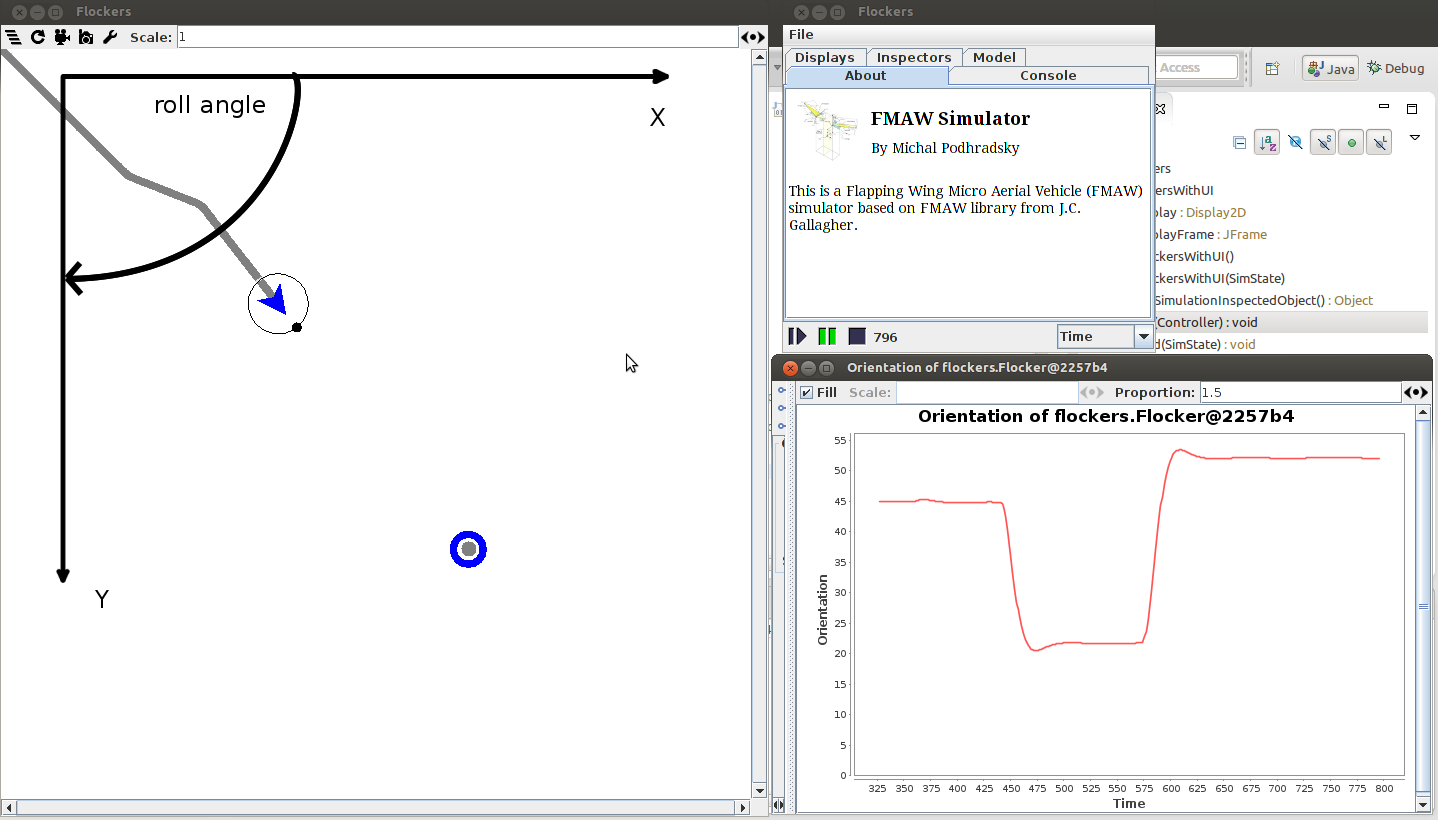
\includegraphics[width=0.85\textwidth]{Files/Figures/simulator.png}
\caption[Screenshot of the simulator]{FWMAV Simulator. \textit{Left:} main window representing the flight area (in our case the water tank), the blue arrow is the FWMAV, the gray trace is the flight path, the blue circle is the desired waypoint (can be repositioned during the flight), the axis labels are only for reference. \textit{Top right:} control window with settings and start/stop/pause button. \textit{Bottom left:} Live plot of simulation data, in this case the orientation of the vehicle.}
\label{fig:simulator}
\end{figure}
